%!TEX program = xelatex
% 完整编译: xelatex -> bibtex -> xelatex -> xelatex
\documentclass[lang=cn,a4paper,cite=authoryear]{elegantpaper}
\songti

\title{\zihao{1}哈尔滨工业大学计算机科学与技术学院 \par 实验报告}
\date{}
% 本文档命令
\usepackage{array}
\usepackage{enumerate}
\usepackage{graphicx}
\usepackage{minted}
\usepackage{subfigure}
\newcommand{\ccr}[1]{\makecell{{\color{#1}\rule{1cm}{1cm}}}}

\begin{document}

\maketitle
\thispagestyle{empty}
\begin{center}
	\zihao{3}
   	{ 课程名称:  机器学习}\\[.5cm]
    { 课程类型:   选修}\\[.5cm]
    { 实验题目:  多项式拟合正弦曲线}\\[.5cm]
	{ 学 号:  1190202110}\\[.5cm]
	{ 姓 名: 田雪洋}\\[.5cm]
    { \date{\zhtoday}}\\[.50cm]
\end{center}


\newpage
\zihao{4}
\section*{\zihao{2}{一、实验目的}}
掌握最小二乘法求解(无惩罚项的损失函数),掌握增加惩罚项(2范数)的损失函数优化,梯度下降法、共轭梯度法,理解过拟合、客服过拟合的方法(如增加惩罚项、增加样本)。

\section*{\zihao{2}{二、实验要求及实验环境}}
\subsection*{\zihao{-2}{1.实验要求}}
1. 生成数据,加入噪声;
\par 2. 用高阶多项式函数拟合曲线;
\par 3. 用解析解求解两种loss的最优解(无正则项和有正则项)
\par 4. 优化方法求解最优解(梯度下降,共轭梯度);
\par 5. 用你得到的实验数据,解释过拟合。
\par 6. 用不同数据量,不同超参数,不同的多项式阶数,比较实验效果。
\par 7. 语言不限,可以用matlab,python。求解解析解时可以利用现成的矩阵求逆。梯度下降,共轭梯度要求自己求梯度,迭代优化自己写。不许用现成的平台,例如pytorch,tensorflow的自动微分工具。

\subsection*{\zihao{-2}{2.实验环境}}
Windows10; python3.8.6;Pycharm 
\section*{\zihao{2}{三、设计思想(本程序中的用到的主要算法及数据结构)}}
对于一个多项式函数
\begin{equation}
	y(x, w)=w_{0}+w_{1} x+\cdots+w_{m} x^{m}=\sum_{i=0}^{m} w_{i} x^{i}
\end{equation}
当$m$足够大时,可以拟合任意曲线,本次实验使用多项式来拟合正弦函数 $sin(2\pi x)$。
\subsection*{\zihao{-2}{1.生成数据}}
首先,先产生若干$x$位于[0,1]的正弦函数 $sin(2\pi x)$的样本,并且给每一个目标值增加一个均值为0,方差为0.09的高斯噪声。代码如下:
\begin{minted}[mathescape,
	numbersep=5pt,
	gobble=2,
	frame=lines,
	framesep=2mm]{Python}
    def data_produce(size,M):
        #在[0,2pi]之间生成size个数据
        x=np.linspace(0,1,size)
        #生成标准差为0.09,均值为0的高斯分布噪声
        gauss_noise=np.random.normal(0,0.09,size=size)
        y=np.sin(2*np.pi*x)
        #生成测试数据集,并添加高斯噪声
        x_train=x
        y_train=y+gauss_noise
        X = []
        for i in range(M + 1):
            X.append(x_train ** i)
            X = np.array(X).T
        return x,y,x_train,y_train,X
\end{minted}
\subsection*{\zihao{-2}{2.最小二乘法(无正则项)}}
采用最小二乘法,即采用如下损失函数来衡量真实值$Y$和预测值$f(x,w)=Xw$之间的误差:
\begin{equation}
	E\left( w \right) =\frac{1}{2}\cdot \left( X\cdot w-Y \right) ^2
\end{equation}
当上述损失函数最小时,即拟合效果最佳。因此,令
\begin{equation}
	\frac{\partial E}{\partial \boldsymbol{w}}=\boldsymbol{X}^{T} \boldsymbol{X} \boldsymbol{w}-\boldsymbol{X}^{T} \boldsymbol{Y}=0
\end{equation}
得到解析解为
\begin{equation}
	\boldsymbol{w}=\left(\boldsymbol{X}^{T} \boldsymbol{X}\right)^{-1} \boldsymbol{X}^{T} \boldsymbol{Y}
\end{equation}
其
$$
\mathbf{X}=\left[\begin{array}{cccc}
	1 & x_{1} & \cdots & x_{1}^{m} \\
	1 & x_{2} & \cdots & x_{2}^{m} \\
	\vdots & \vdots & \ddots & \vdots \\
	1 & x_{N} & \cdots & x_{N}^{m}
\end{array}\right]
$$
这样,便可以编程得到参数$w$的取值,进而求得$f(x,w)$函数。这便是最小二乘法拟合的思想。代码如下:
\begin{minted}[mathescape,
	numbersep=5pt,
	gobble=2,
	frame=lines,
	breaklines,
	framesep=2mm]{Python}
    def lsm(X,y_train,lamda):
        #最小二乘法得到多项式函数的参数w,lamda即正则项的超参数,
        #当lamda=0时,为无正则项的最小二乘法算法,
        #当lamda!=0时,为带正则项的最小二乘法算法。
        w=np.dot(np.dot(np.linalg.inv(np.dot(X.T,X)
    +   lamda*np.eye(X.shape[1])),X.T),y_train)
        #求得多项式函数的解析式为:
        pre=np.poly1d(w[::-1])
        return w,pre
    def loss(X,y_train,w,lamda):
        #计算损失函数E(w)
        return 1/2*np.dot((X.dot(w)-y_train).T,(X.dot(w)-y_train))
        +0.5*lamda*np.dot(w.T,w)
\end{minted}

\subsection*{\zihao{-2}{3.最小二乘法(含正则项)}}
通常使用最小二乘法拟合时,可能出现过拟合的现象。因此为了避免过拟合的出现,我们在通常在误差函数上加上惩罚项来避免过拟合的出现。
因此,我们得到了
\begin{equation}
	E\left( w \right) =\frac{1}{2}\cdot \left( X\cdot w-Y \right) ^2
\end{equation}
对上述式子求偏导得到
\begin{equation}
\frac{\partial \widetilde{E}}{\partial \boldsymbol{w}}=\boldsymbol{X}^{T} \boldsymbol{X} \boldsymbol{w}-\boldsymbol{X}^{T} \boldsymbol{Y}+\lambda \boldsymbol{w}
\end{equation}
令偏导数等于0求得$w$为
\begin{equation}
\boldsymbol{w}=\left(\boldsymbol{X}^{T} \boldsymbol{X}+\lambda\right)^{-1} \boldsymbol{X}^{T} \boldsymbol{Y}
\end{equation}
代码和无正则项的代码相同,参数lamda即正则项的超参数$\lambda$,当lamda=0时,为无正则项的最小二乘法算法,当lamda!=0时,为带正则项的最小二乘法算法。
\subsection*{\zihao{-2}{4.梯度下降法}}
梯度下降法是用来计算函数最小值的。它和下山的过程很像,采用逐步逼近的方式求取极值。梯度下降法首先在函数上随机选定一点,然后计算该点的梯度。因为梯度的方向就是函数之变化最快的方向,所以沿着梯度下降最快的方向前进,逐步逼近函数的极值点。在本次实验中,即使损失函数最小,并且记录当前的$w$。
\par 对于式子(6),我们设置学习速率$\alpha$和迭代次数。$w$的迭代方程为
\begin{equation}
	\boldsymbol{w}=\boldsymbol{w}-\alpha \cdot \frac{\partial \widetilde{E}}{\partial \boldsymbol{w}}
\end{equation}
由于是采用设置迭代次数的方式,所以当新的损失函数大于原来的损失函数时,说明已经过来极值点了,此时,将学习速率减半,重新迭代,直到完成迭代次数。
代码如下:
\begin{minted}[mathescape,
	numbersep=5pt,
	gobble=2,
	frame=lines,
	breaklines,
	framesep=2mm]{Python}
   def Gradient_descent(X,y_train,deta,lamda,times):
       #梯度下降法
       #设置初始的w的值
       w=np.zeros(X.shape[1])
       w0=w
       #计算初始的损失函数的取值
       loss_0=loss(X,y_train,w,lamda)
       #根据设置的迭代次数,进行迭代
       for i in range(1,times+1):
            #E(w)对w求偏导
            gradient=((X.T).dot(X)).dot(w)-np.dot(X.T,y_train)+lamda*w
            #w的迭代方程,deta为学习速率
            w=w-deta*gradient
            #计算新的损失函数
            loss_new=loss(X,y_train,w,lamda)
            #当损失函数变大时,学习速率减半
            if(loss_new<loss_0):
                loss_0=loss_new
                w0=w
            else:
                deta=deta*0.5
        #得到多项式函数
        pre = np.poly1d(w0[::-1])
        return w0,pre,loss_0
\end{minted}
\subsection*{\zihao{-2}{5.共轭梯度法}}
共轭梯度法是用来求解线性方程$Ax=b$。但共轭梯度法并不能用来解任意的线性方程。它要求系数矩阵是对称且正定的矩阵。根据式(6),显然该结果是符合要求的。因此首先令
\begin{equation}
	A=X^T\cdot X+\lambda \cdot I , B=X^T\cdot Y
\end{equation}
然后令$r_{0}=A x_{0}-b, p_{0}=-r_{0}$。接着,得到如下算法:
\begin{equation}
\begin{aligned}
	\alpha _k&=\frac{r_{k}^{T}r_k}{p_{k}^{T}Ap_k}\\
	w_{k+1}&=w_k+\alpha _kp_k\\
	r_{k+1}&=r_k+\alpha _kAp_k\\
	\beta _{k+1}&=\frac{r_{k+1}^{T}r_{k+1}}{r_{k}^{T}r_k}\\
	p_{k+1}&=-r_{k+1}+\beta _{k+1}p_k\\
\end{aligned}
\end{equation}
该算法一直执行,直到$r_{k}^{T}r_k$不满足设定的精度。代码如下:
\begin{minted}[mathescape,
	numbersep=5pt,
	gobble=2,
	frame=lines,
	breaklines,
	framesep=2mm]{Python}
   def Conjugate_gradient(X,y_train,lamda,epsilon):
        #共轭梯度法
        #计算A,b
        A=X.T.dot(X)+lamda*np.eye(X.shape[1])
        b=X.T.dot(y_train)
        #初始化w,r,p,将rkT*rk保留
        w = np.zeros(X.shape[1])
        r=A.dot(w)-b
        p=-r
        t=r.T.dot(r)
        #循环,直到t不满足精度为止
        while t>epsilon:
            #算法迭代
            alpha=t/p.T.dot(A).dot(p)
            w=w+alpha*p
            r=r+alpha*A.dot(p)
            beta=r.T.dot(r)/t
            p=-r+beta*p
            t=r.T.dot(r)
        #得到多项式函数的解析式
        pre = np.poly1d(w[::-1])
        return w,pre
\end{minted}


\section*{\zihao{2}{四、实验结果与分析}}
\subsection*{\zihao{-2}{1.无正则项的解析解}}
当训练集的数据量为10时,不同阶数的拟合效果:
\begin{itemize}
	\item 拟合函数解析为一次函数
	\begin{figure}[H]
		\centering
		
\includegraphics[scale=0.5]{1}
	\end{figure}
	\item 拟合函数解析为三次函数
	\begin{figure}[H]
		\centering
		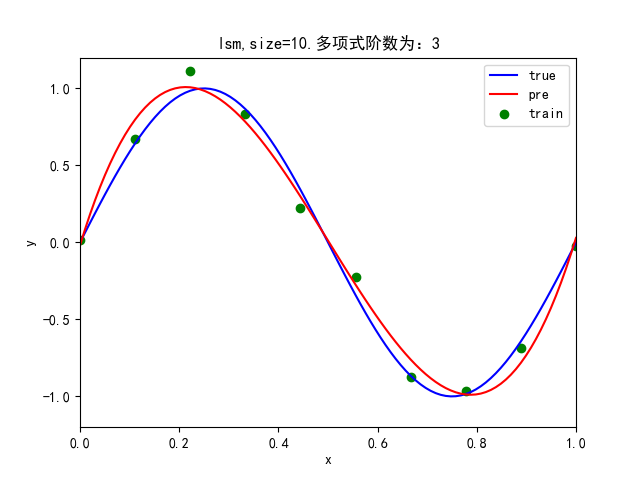
\includegraphics[scale=0.5]{3}
	\end{figure}
	\item 拟合函数解析为五次函数
	\begin{figure}[H]
		\centering
		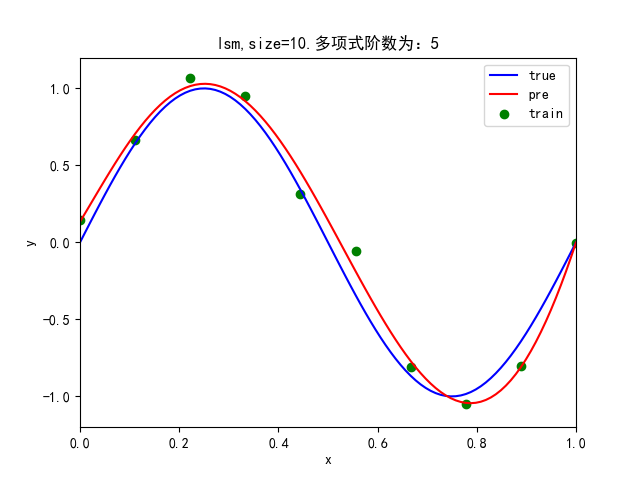
\includegraphics[scale=0.5]{5}
	\end{figure}
    \item 拟合函数解析为七次函数
    \begin{figure}[H]
    	\centering
    	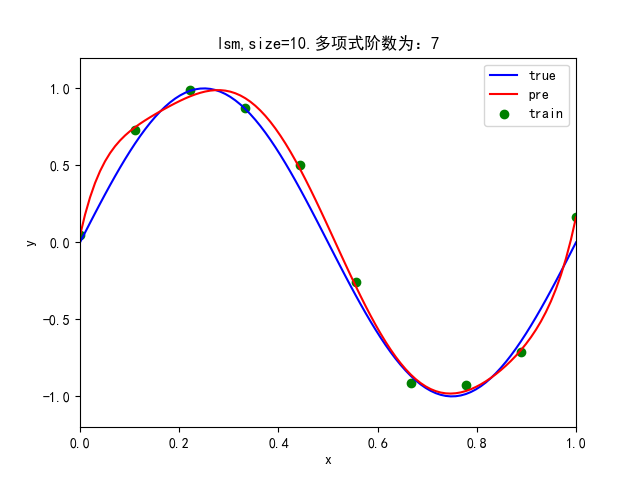
\includegraphics[scale=0.5]{7}
    \end{figure}
    \item 拟合函数解析为九次函数
    \begin{figure}[H]
    	\centering
    	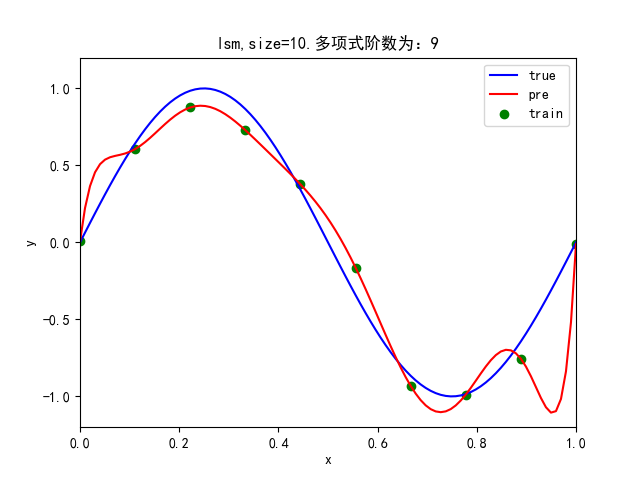
\includegraphics[scale=0.5]{9}
    \end{figure}
    \item 拟合函数解析为十九次函数
    \begin{figure}[H]
    	\centering
    	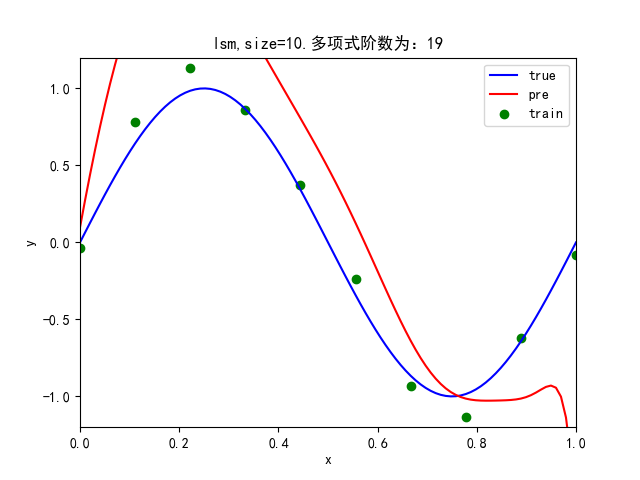
\includegraphics[scale=0.5]{19}
    \end{figure}
\end{itemize}
可以看到,拟合函数为一次函数时,预测函数和原函数差别较大,基本无法拟合,此时明显为欠拟合的状态。当拟合函数的次数为3次,5次时拟合效果已经很好了,预测曲线和原曲线已经基本上重合,此时的方根均值分别为:0.0545和
0.0177,拟合效果极佳。但是,当拟合函数的次数增加到7次以后,7次函数和9次函数已经全部穿过了测试点,但是可以看到,曲线已经比原曲线相差甚远,已经开始扭曲了,当次数继续增加到19次时,预测曲线已经彻底扭曲,和原曲线相差越来越大,过拟合的现象越来越严重。
当我们逐渐增加训练集的样本数量时,对于九次函数结果如下:
\begin{itemize}
	\item 训练集样本容量为30
	\begin{figure}[H]
		\centering
		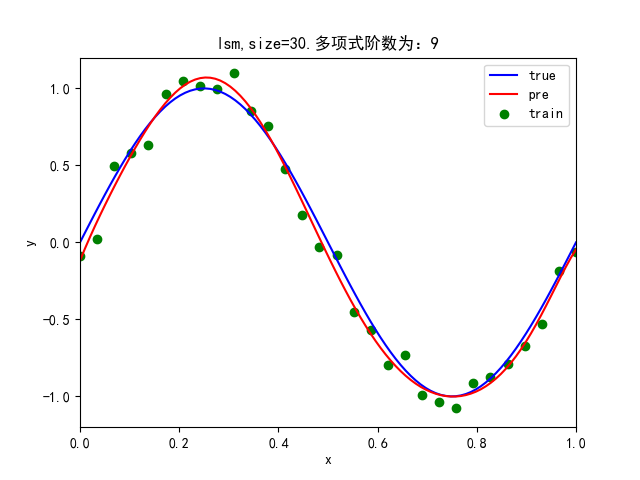
\includegraphics[scale=0.5]{30}
	\end{figure}
\item 训练集样本容量为50
\begin{figure}[H]
	\centering
	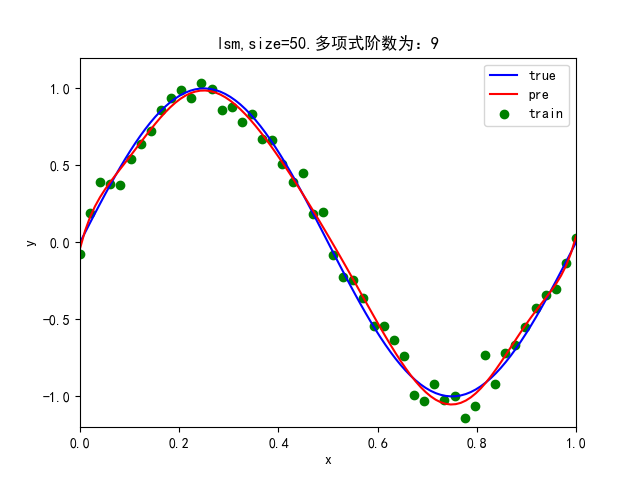
\includegraphics[scale=0.5]{50}
\end{figure}
\item 训练集样本容量为100
\begin{figure}[H]
	\centering
	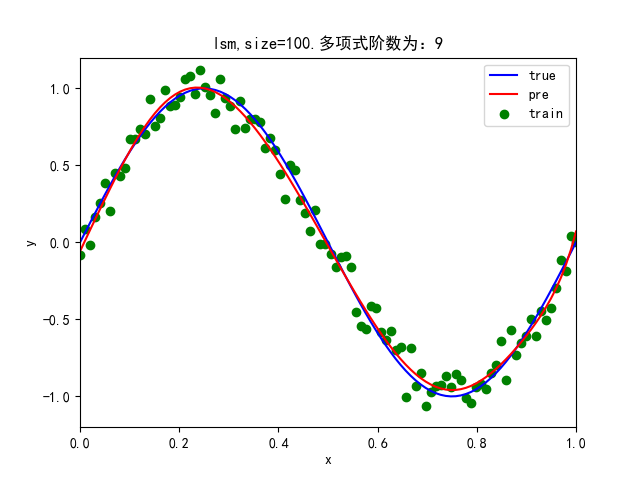
\includegraphics[scale=0.5]{100}
\end{figure}

\end{itemize}
可以看到,随着样本容量的增加,曲线的拟合效果越来越好,这说明:增加训练集样本容量可以消除过拟合现象。
\subsection*{\zihao{-2}{2.含正则项的解析解}}
不仅增加样本容量可以消除过拟合现象,增加正则项同样可以消除过拟合现象,下面我们研究不同取值的参数对拟合效果的影响。我们将使用均方根来评价不同参数取值的拟合效果。
其中训练集的样本容量为10,验证集样本容量为20,多项式的阶数为9,多次运行的拟合效果如下:
\begin{figure}[H]
	\centering
	
	\subfigure[pic1.]{
		\begin{minipage}[t]{0.5\linewidth}
			\centering
			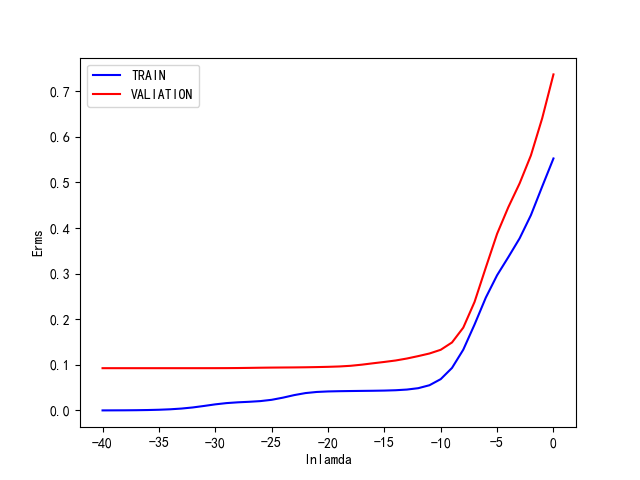
\includegraphics[scale=0.4]{erm1}
		\end{minipage}%
	}%
	\subfigure[pic2.]{
		\begin{minipage}[t]{0.5\linewidth}
			\centering
			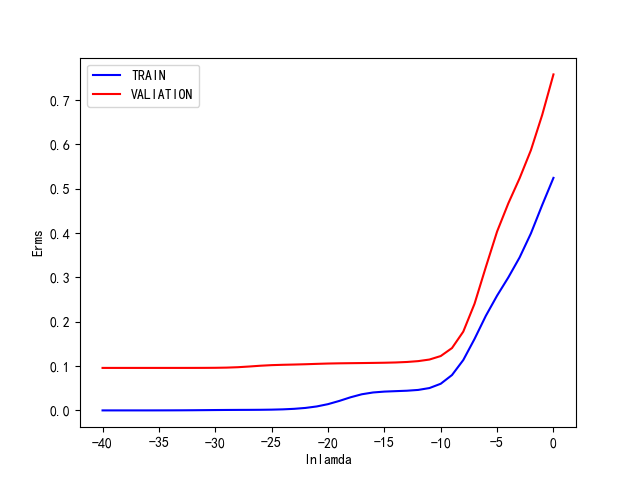
\includegraphics[scale=0.4]{erm2}
		
		\end{minipage}%
	}%
	%这个回车键很重要 \quad也可以
	\quad
\subfigure[pic3.]{
	\begin{minipage}[t]{0.5\linewidth}
		\centering
		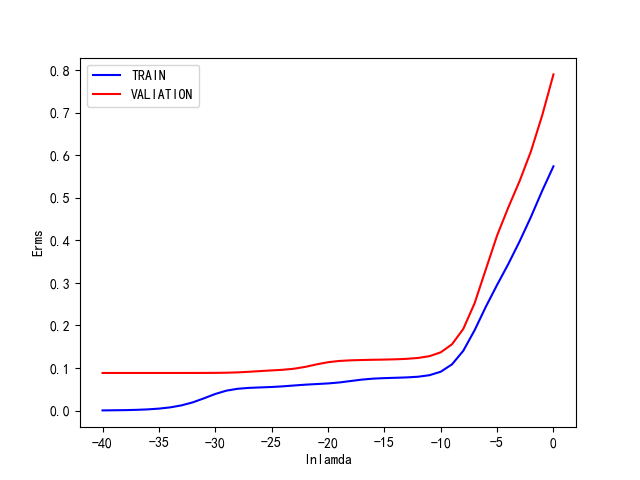
\includegraphics[scale=0.4]{erm3}
	
	\end{minipage}
}%
\subfigure[pic4.]{
	\begin{minipage}[t]{0.5\linewidth}
		\centering
		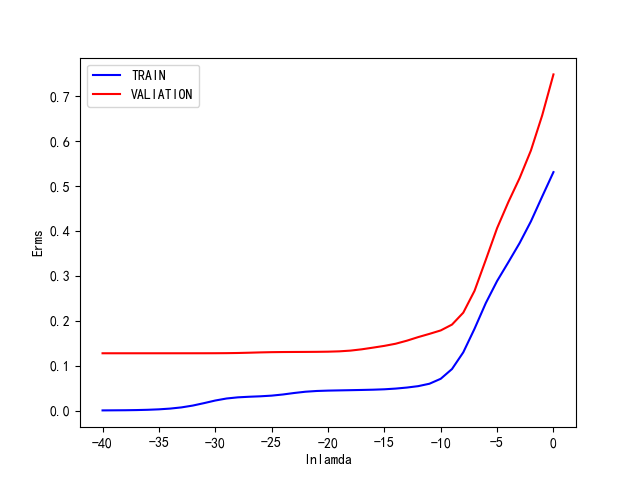
\includegraphics[scale=0.4]{erm4}

	\end{minipage}
}%

\centering
\end{figure}
可以看到,当参数lamda在$\left(e^{-40}, e^{-10}\right)$之间时均方差几乎保持不变,且训练集的接近0,在测试集上保持稳定。
故取$\lambda =e^{-30}$时,把在训练集样本容量为10,阶数为9的条件下的带正则项和不带正则项的最小二乘法拟合的图像进行比较。
    \begin{figure}[H]
	\centering
	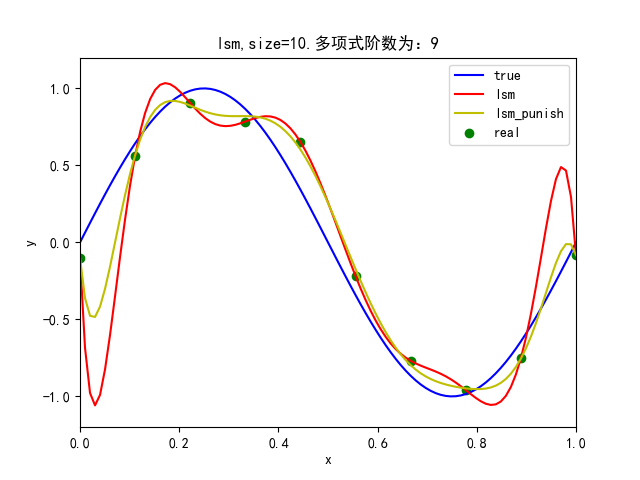
\includegraphics[scale=0.5]{10}
\end{figure}
可以看到,加入正则项后的确有助于减轻过拟合现象,提高拟合效果。
\subsection*{\zihao{-2}{3.梯度下降法求得优化解}}
取$\lambda =e^{-12}$时,使用梯度下降法,初始学习速率为0.01,迭代100000次,训练集的样本容量为10,得到的不同阶数下的拟合图像如下
\begin{itemize}
	\item 拟合函数解析为一次函数
	\begin{figure}[H]
		\centering
		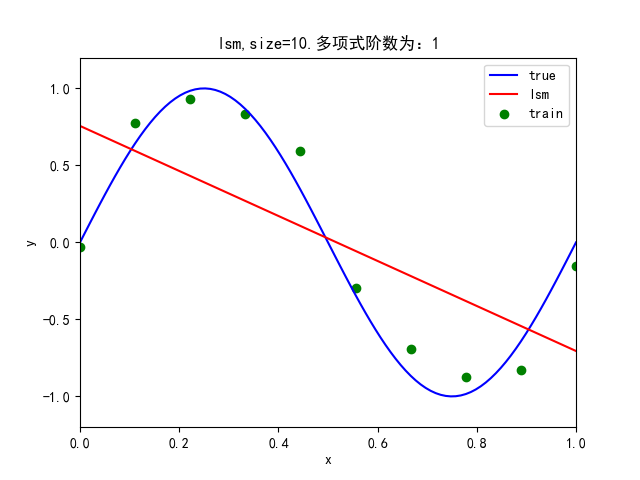
\includegraphics[scale=0.5]{g1}
	\end{figure}
	\item 拟合函数解析为三次函数
	\begin{figure}[H]
		\centering
		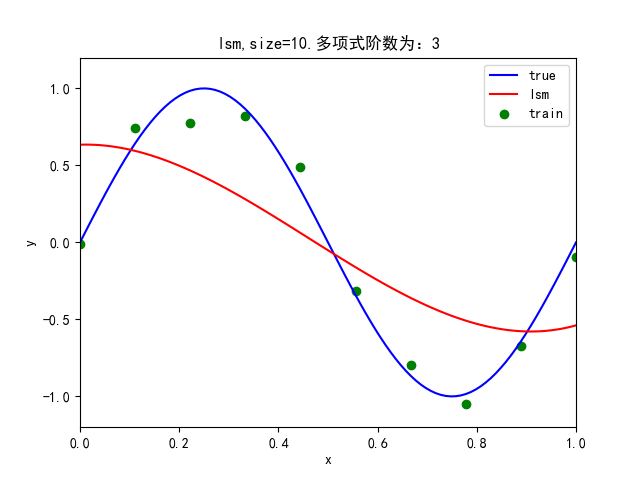
\includegraphics[scale=0.5]{g3}
	\end{figure}
	\item 拟合函数解析为五次函数
	\begin{figure}[H]
		\centering
		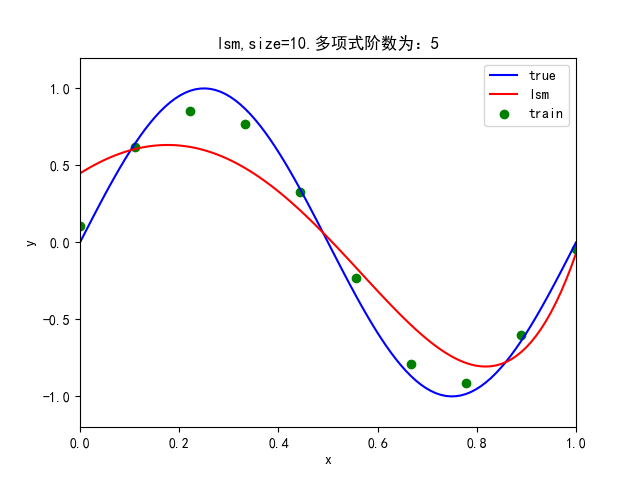
\includegraphics[scale=0.5]{g5}
	\end{figure}
	\item 拟合函数解析为七次函数
	\begin{figure}[H]
		\centering
		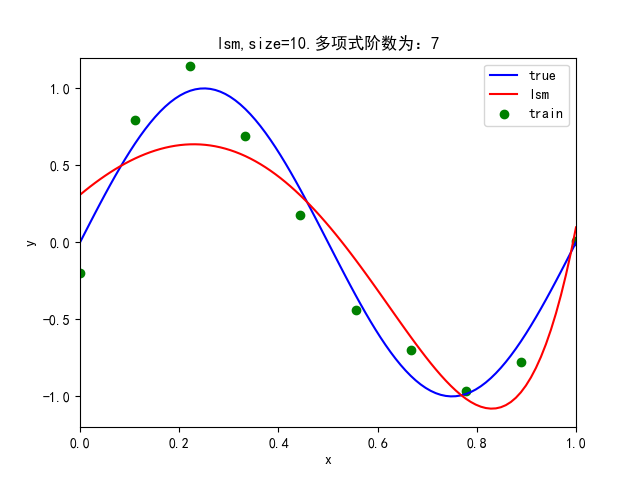
\includegraphics[scale=0.5]{g7}
	\end{figure}
	\item 拟合函数解析为九次函数
	\begin{figure}[H]
		\centering
		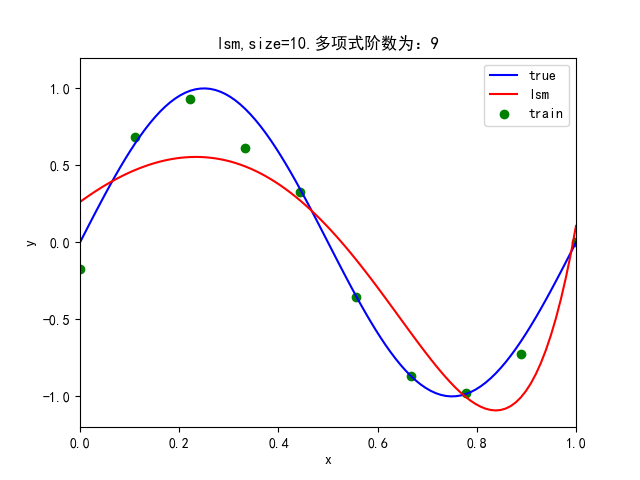
\includegraphics[scale=0.5]{g9}
	\end{figure}
	\item 拟合函数解析为十九次函数
	\begin{figure}[H]
		\centering
		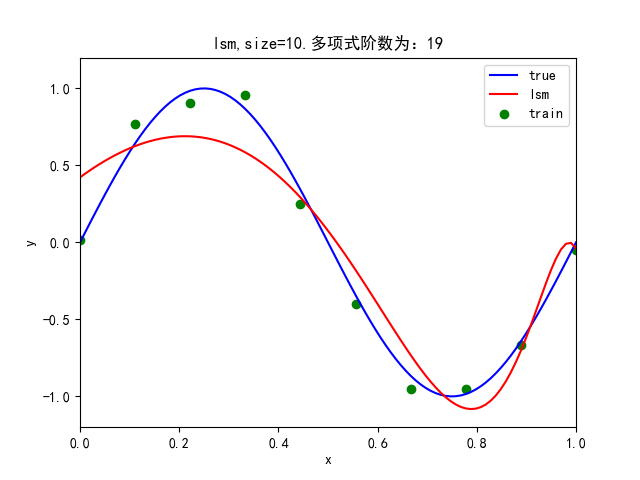
\includegraphics[scale=0.5]{g19}
	\end{figure}
\end{itemize}
当固定拟合函数的阶数为9,训练集的样本容量增大,得到的结果如下
\begin{itemize}
	\item 训练集样本容量为30
	\begin{figure}[H]
		\centering
		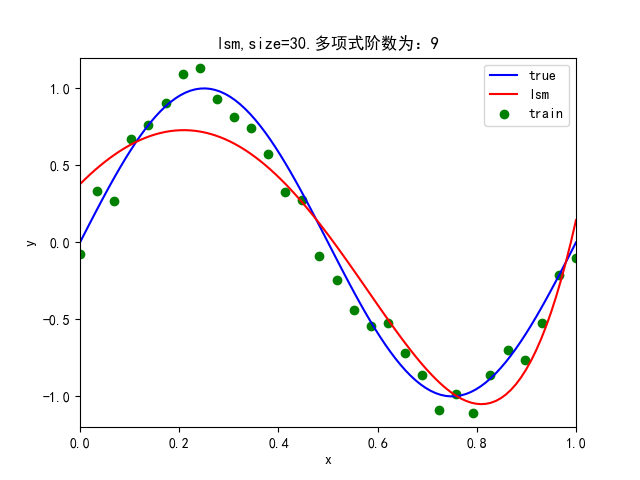
\includegraphics[scale=0.5]{g30}
	\end{figure}
	\item 训练集样本容量为50
	\begin{figure}[H]
		\centering
		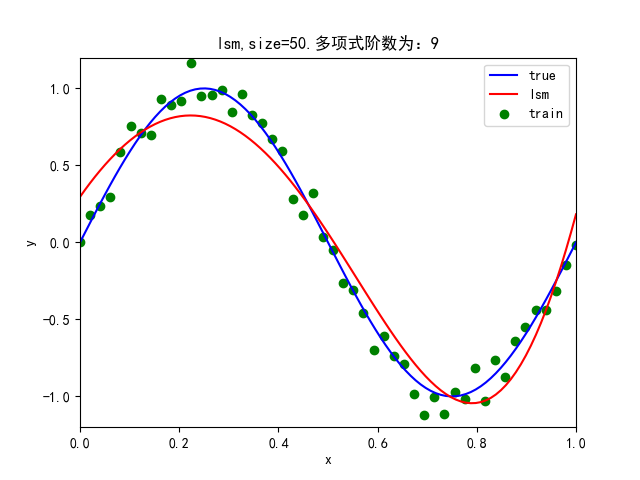
\includegraphics[scale=0.5]{g50}
	\end{figure}
	\item 训练集样本容量为100
	\begin{figure}[H]
		\centering
		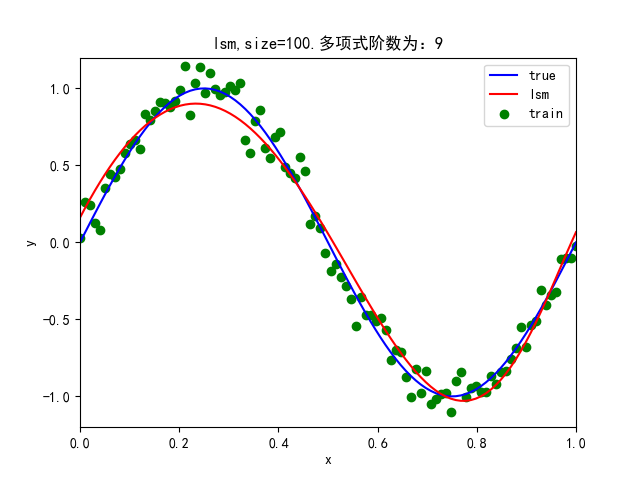
\includegraphics[scale=0.5]{g100}
	\end{figure}
	
\end{itemize}
可以看到,在样本容量较少时,梯度下降法的效果不是很理想,远不如最小二乘法,但随着样本容量的增大,梯度下降法的拟合效果逐渐变优。
\subsection*{\zihao{-2}{4.共轭梯度法求得优化解}}
取$\lambda =e^{-10}$时,使用共轭梯度法,精度为$e^{-6}$,训练集的样本容量为10,得到的不同阶数下的拟合图像如下
\begin{itemize}
	\item 拟合函数解析为一次函数
	\begin{figure}[H]
		\centering
		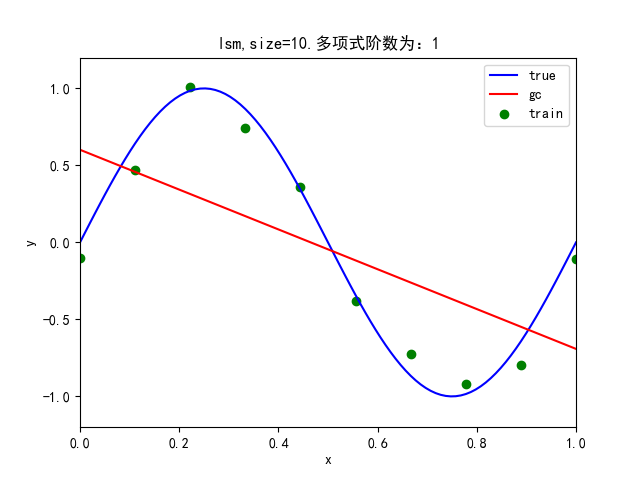
\includegraphics[scale=0.5]{gc1}
	\end{figure}
	\item 拟合函数解析为三次函数
	\begin{figure}[H]
		\centering
		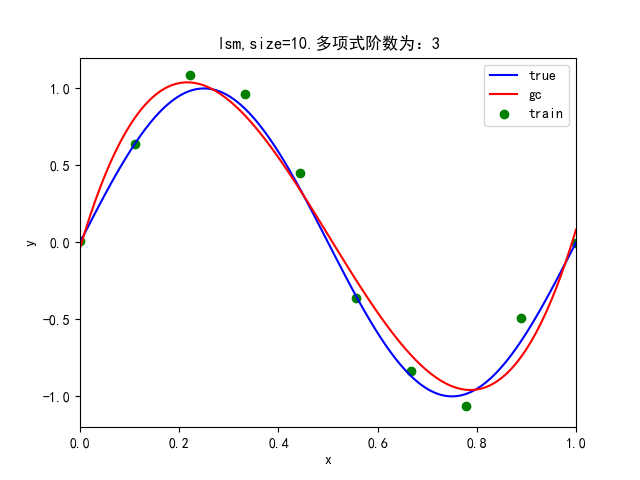
\includegraphics[scale=0.5]{gc3}
	\end{figure}
	\item 拟合函数解析为五次函数
	\begin{figure}[H]
		\centering
		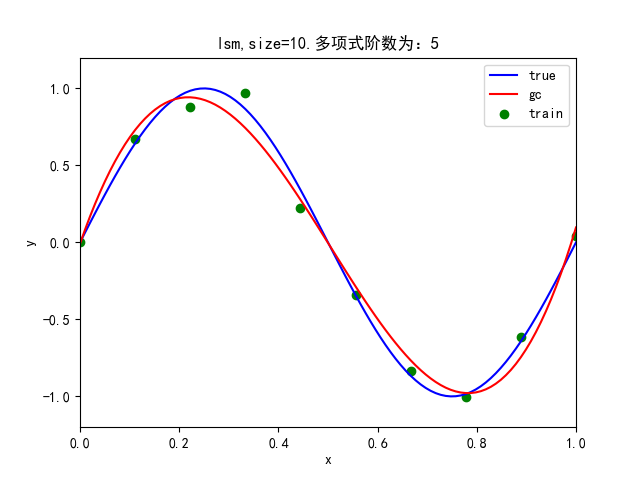
\includegraphics[scale=0.5]{gc5}
	\end{figure}
	\item 拟合函数解析为七次函数
	\begin{figure}[H]
		\centering
		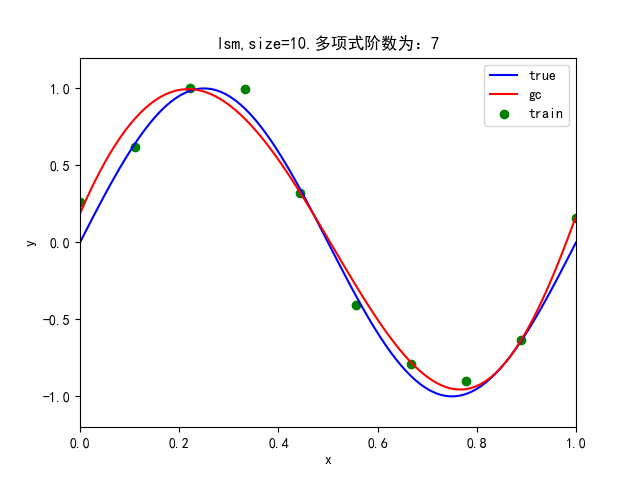
\includegraphics[scale=0.5]{gc7}
	\end{figure}
	\item 拟合函数解析为九次函数
	\begin{figure}[H]
		\centering
		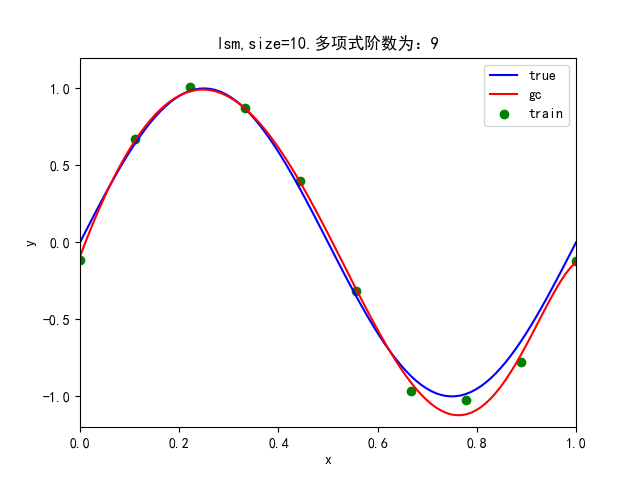
\includegraphics[scale=0.5]{gc9}
	\end{figure}
	\item 拟合函数解析为十九次函数
	\begin{figure}[H]
		\centering
		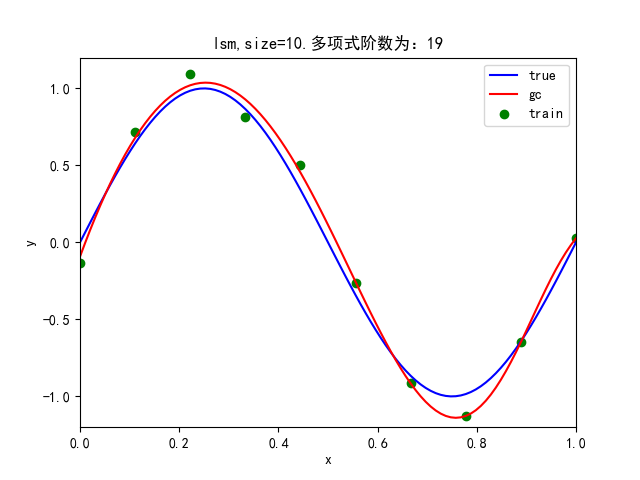
\includegraphics[scale=0.5]{gc19}
	\end{figure}
\end{itemize}
当我们逐渐增加训练集的样本数量时,对于九次函数结果如下:
\begin{itemize}
	\item 训练集样本容量为30
	\begin{figure}[H]
		\centering
		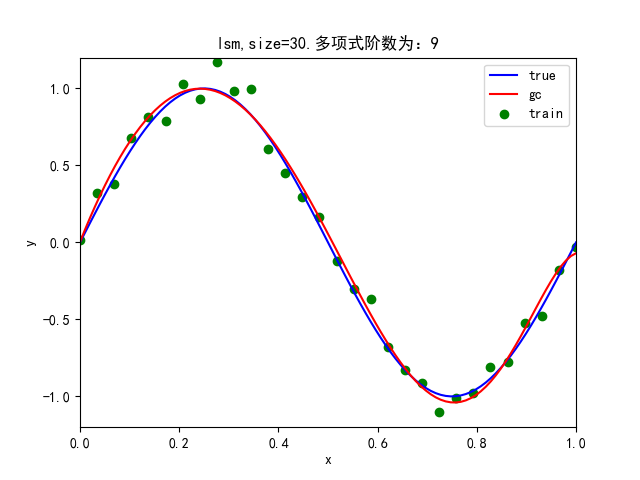
\includegraphics[scale=0.5]{gc30}
	\end{figure}
	\item 训练集样本容量为50
	\begin{figure}[H]
		\centering
		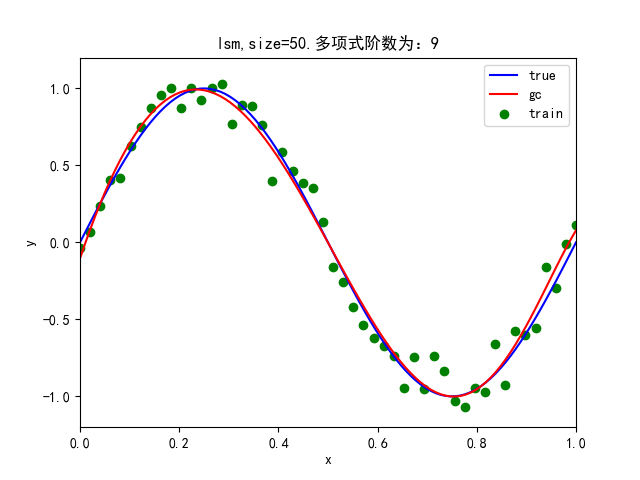
\includegraphics[scale=0.5]{gc50}
	\end{figure}
	\item 训练集样本容量为100
	\begin{figure}[H]
		\centering
		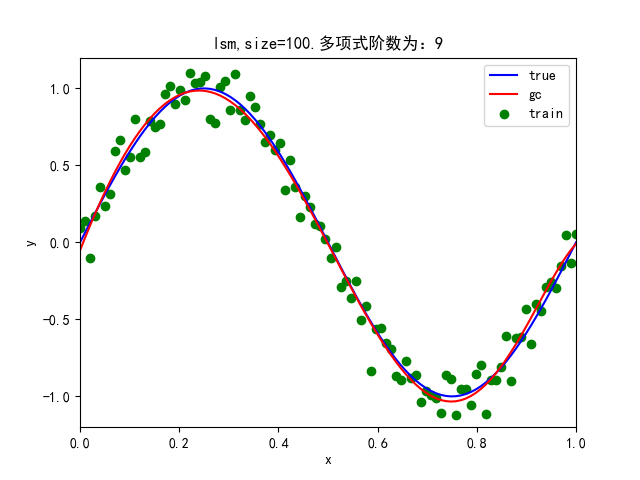
\includegraphics[scale=0.5]{gc100}
	\end{figure}
	
\end{itemize}
可以看到,随着样本容量的增加,曲线的拟合效果越来越好。
\subsection*{\zihao{-2}{5.四种方法拟合对比}}
通过对上面的图像分析可以得到。在上面的四种方法中,最小二乘法带正则项的拟合效果最好,其次是不带正则项的最小二乘法和共轭梯度法。梯度下降法在样本容量较小时拟合效果较差,但随着样本容量的提升,梯度下降法的拟合效果也在逐渐变好。
\section*{\zihao{2}{五、结论}}
在本次实验的多项式函数拟合中,我们可以看到多项式的次数越高,拟合效果越好,但是可能会出现过拟合的现象,但是我们可以通过增加样本容量和正则项的方法来减轻过拟合现象。
\par 这过拟合现象出现的原因是由于样本数量少但拟合能力过强,导致拟合结果过分依赖已知的,少量的数据,其泛化能力减弱造成的,这种过强的拟合效果无法拟合出正弦曲线,其曲线会因尽量穿过已知点而被过分扭曲。所以增大样本容量可以减轻过拟合现象的出现,甚至消除。另一方面,在拟合函数中加入参数的正则项后,过拟合现象得到减轻。这是因为当参数数量变多时,模型的复杂度降低,从而使之与目标曲线相适应。因此,增加正则项是减轻过拟合现象的手段之一。

\par 梯度下降法相比共轭梯度收敛速度很慢,迭代次数很大,而且性能较差。但共轭梯度法适用条件更差,它必须要求线性方程的系数矩阵正定且对称,因此它的适用范围更小。但是若是满足条件,共轭梯度法的性能要明显高于梯度下降法。

\section*{\zihao{2}{六、参考文献}}

\section*{\zihao{2}{七、附录:源代码(带注释)}}
\subsection*{\zihao{-2}{exp1.py}} 
\begin{minted}[
	numbersep=3pt,
	linenos,
	frame=lines,
	breaklines,
	framesep=2mm]{Python}
import math

import pandas as pd
import numpy as np
import matplotlib.pyplot as plt
from sklearn.model_selection import train_test_split


def data_produce(size,M):
    #在[0,2pi]之间生成size个数据
    x=np.linspace(0,1,size)
    #生成标准差为0.09,均值为0的高斯分布噪声
    gauss_noise=np.random.normal(0,0.09,size=size)
    y=np.sin(2*np.pi*x)
    #生成测试数据集,并添加高斯噪声
    x_train=x
    y_train=y+gauss_noise
    X = []
    for i in range(M + 1):
        X.append(x_train ** i)
        X = np.array(X).T
    return x,y,x_train,y_train,X
def lsm(X,y_train,lamda):
    # 最小二乘法得到多项式函数的参数w,lamda即正则项的超参数,
    # 当lamda=0时,为无正则项的最小二乘法算法,
    # 当lamda!=0时,为带正则项的最小二乘法算法。
    w=np.dot(np.dot(np.linalg.inv(np.dot(X.T,X)+lamda*np.eye(X.shape[1])),X.T),y_train)
    #求得多项式函数的解析式为:
    pre=np.poly1d(w[::-1])
    return w,pre
    def loss(X,y_train,w,lamda):
    #计算损失函数E(w)
    return 1/2*np.dot((X.dot(w)-y_train).T,(X.dot(w)-y_train))+lamda/2*np.dot(w.T,w)
def ERMS(loss,size):
    #计算方根均值Erms
    return np.sqrt(2 * loss / size)
def Gradient_descent(X,y_train,deta,lamda,times):#梯度下降法
    #设置初始的w的值
    w=np.zeros(X.shape[1])
    w0=w
    #计算初始的损失函数的取值
    loss_0=loss(X,y_train,w,lamda)
    #根据设置的迭代次数,进行迭代
    for i in range(1,times+1):
        #E(w)对w求偏导
        gradient=((X.T).dot(X)).dot(w)-np.dot(X.T,y_train)+lamda*w
        #w的迭代方程,deta为学习速率
        w=w-deta*gradient
        #计算新的损失函数
        loss_new=loss(X,y_train,w,lamda)
        #当损失函数变大时,学习速率减半
        if(loss_new<loss_0):
            loss_0=loss_new
             w0=w
        else:
             deta=deta*0.5
    #得到多项式函数
    pre = np.poly1d(w0[::-1])
    return w0,pre,loss_0
def Conjugate_gradient(X,y_train,lamda,epsilon):
    #共轭梯度法
    #计算A,b
    A=X.T.dot(X)+lamda*np.eye(X.shape[1])
    b=X.T.dot(y_train)
    #初始化w,r,p,将rkT*rk保留
    w = np.zeros(X.shape[1])
    r=A.dot(w)-b
    p=-r
    t=r.T.dot(r)
    #循环,直到t不满足精度为止
    while t>epsilon:
    #算法迭代
        alpha=t/p.T.dot(A).dot(p)
        w=w+alpha*p
        r=r+alpha*A.dot(p)
        beta=r.T.dot(r)/t
        p=-r+beta*p
        t=r.T.dot(r)
        #得到多项式函数的解析式
    pre = np.poly1d(w[::-1])
    return w,pre
def plot_lsm(size,lamda,a):
    #生成数据集
    x,y,x_train,y_train,X=data_produce(size,a)
    #最小二乘法预测
    w,pre=lsm(X,y_train,lamda)
    w_loss,pre_loss=lsm(X,y_train,math.exp(-30))
    #打印方差均根
    print(ERMS(loss(X,y_train,w,lamda),size))
    print(pre)
    plt.xlabel("x")
    plt.ylabel("y")
    plt.xlim(0,1)
    plt.ylim(-1.2,1.2)
    plt.rcParams['font.sans-serif'] = ['SimHei']
    plt.rcParams['axes.unicode_minus'] = False
    plt.title("lsm,size="+str(size)+".多项式阶数为:"+str(a))
    x = np.linspace(0, 1, 100)
    y = np.sin(x * 2 * np.pi)
    plt.plot(x,y,color='b',label='true')
    plt.scatter(x_train,y_train,color='g',label='real')
    plt.plot(x,pre(x),color='r',label='lsm')
    plt.plot(x, pre_loss(x),color='y' ,label='lsm_punish')
    plt.legend()
    plt.savefig(str(size)+".png")
def plot_lsm_lamda(size,a=9):
    x,y,x_train1,y1_train,x_train=data_produce(size,a)
    x, y, x_test1, y1_test, x_test = data_produce(size*2,a)
    # 划分数据集为测试集,训练集,验证集
    #x_train, x_test, y1_train, y1_test = train_test_split(X, y_train, random_state=1, test_size=10)
    lamda=np.linspace(-40,0,40).astype(int)
    ERMtest=[]
    ERMtrain=[]
    #对于测试集和预测集分别计算均方根误差
    for i in lamda:
        t=math.exp(i)
        w_test,pre=lsm(x_test,y1_test,t)
        ERMtest.append(ERMS(loss(x_test,y1_test,w_test,t),size))
        w_train, pre = lsm(x_train, y1_train, t)
        ERMtrain.append(ERMS(loss(x_train, y1_train, w_train, t), size))
    plt.xlabel("lnlamda")
    plt.ylabel("Erms")
    plt.rcParams['font.sans-serif'] = ['SimHei']
    plt.rcParams['axes.unicode_minus'] = False
    minERM=1.0
    minlamda=0
    #找出均方根误差最小值
    for i in range(0,len(ERMtest)):
        if minERM>=ERMtest[i]:
            minERM=ERMtest[i]
            minlamda=lamda[i]
    print(minERM)
    plt.plot(lamda,ERMtrain,color='b',label='TRAIN')
    plt.plot(lamda,ERMtest,color='r',label='VALIATION')
    plt.legend()
    plt.savefig("erm4.png")
def plot_Gu(size,lamda,a):
    #生成数据集
    x,y,x_train,y_train,X=data_produce(size,a)
    #梯度下降法
    times=10000
    w,pre,loss_0=Gradient_descent(X,y_train,0.01,lamda,times)
    #打印方差均根
    print(ERMS(loss_0,size))
    print(pre)
    plt.xlabel("x")
    plt.ylabel("y")
    plt.xlim(0,1)
    plt.ylim(-1.2,1.2)
    plt.rcParams['font.sans-serif'] = ['SimHei']
    plt.rcParams['axes.unicode_minus'] = False
    plt.title("lsm,size="+str(size)+".多项式阶数为:"+str(a))
    x = np.linspace(0, 1, 100)
    y = np.sin(x * 2 * np.pi)
    plt.plot(x,y,color='b',label='true')
    plt.scatter(x_train,y_train,color='g',label='train')
    plt.plot(x,pre(x),color='r',label='lsm')
    plt.legend()
    #plt.show()
    plt.savefig("g"+str(size)+".png")
def plot_Gc(size,lamda,a):
    #生成数据集
    x,y,x_train,y_train,X=data_produce(size,a)
    #共轭梯度法
    w,pre=Conjugate_gradient(X,y_train,lamda,1e-6)
    #打印方差均根
    print(ERMS(loss(X,y_train,w,lamda),size))
    print(pre)
    plt.xlabel("x")
    plt.ylabel("y")
    plt.xlim(0,1)
    plt.ylim(-1.2,1.2)
    plt.rcParams['font.sans-serif'] = ['SimHei']
    plt.rcParams['axes.unicode_minus'] = False
    plt.title("lsm,size="+str(size)+".多项式阶数为:"+str(a))
    x = np.linspace(0, 1, 100)
    y = np.sin(x * 2 * np.pi)
    plt.plot(x,y,color='b',label='true')
    plt.scatter(x_train,y_train,color='g',label='train')
    plt.plot(x,pre(x),color='r',label='gc')
    plt.legend()
    #plt.show()
    plt.savefig("gc"+str(size)+".png")
\end{minted}
\subsection*{\zihao{-2}{main1.py}} 
\begin{minted}[mathescape,
	numbersep=5pt,
	frame=lines,
	breaklines,
	linenos,
	framesep=2mm]{Python}
import math

import exp1
import numpy as np
import matplotlib.pyplot as plt
#不带正则项的最小二乘法的解析解
#样本容量为10
# exp1.plot_lsm(size=10,lamda=0,a=1)#一次函数
#exp1.plot_lsm(size=10,lamda=0,a=3)#三次函数
#exp1.plot_lsm(size=10,lamda=0,a=5)#五次函数
#exp1.plot_lsm(size=10,lamda=0,a=7)#七次函数
#exp1.plot_lsm(size=10,lamda=0,a=9)#九次函数
#exp1.plot_lsm(size=10,lamda=0,a=19)#十九次函数
#样本容量为30
#exp1.plot_lsm(size=30,lamda=0,a=9)#九次函数
#样本容量为50
#exp1.plot_lsm(size=50,lamda=0,a=9)#九次函数
#样本容量为100
#exp1.plot_lsm(size=100,lamda=0,a=9)#九次函数
#带正则项的最小二乘法的解析解
#exp1.plot_lsm_lamda(10)
#梯度下降法不同阶数
#exp1.plot_Gu(size=10,lamda=math.exp(-12),a=1)#一次函数
#exp1.plot_Gu(size=10,lamda=math.exp(-12),a=3)#三次函数
#exp1.plot_Gu(size=10,lamda=math.exp(-12),a=5)#五次函数
#exp1.plot_Gu(size=10,lamda=math.exp(-12),a=7)#七次函数
#exp1.plot_Gu(size=10,lamda=math.exp(-12),a=9)#九次函数
#exp1.plot_Gu(size=10,lamda=math.exp(-12),a=19)#十九次函数
#样本容量为30
#exp1.plot_Gu(size=30,lamda=math.exp(-12),a=9)#九次函数
#样本容量为50
#exp1.plot_Gu(size=50,lamda=math.exp(-12),a=9)#九次函数
#样本容量为100
#exp1.plot_Gu(size=100,lamda=math.exp(-12),a=9)#九次函数
#共轭梯度法
#exp1.plot_Gc(size=10,lamda=math.exp(-10),a=1)#一次函数
#exp1.plot_Gc(size=10,lamda=math.exp(-10),a=3)#三次函数
#exp1.plot_Gc(size=10,lamda=math.exp(-10),a=5)#五次函数
#exp1.plot_Gc(size=10,lamda=math.exp(-10),a=7)#七次函数
#exp1.plot_Gc(size=10,lamda=math.exp(-10),a=9)#九次函数
#exp1.plot_Gc(size=10,lamda=math.exp(-10),a=19)#十九次函数
#样本容量为30
#exp1.plot_Gc(size=30,lamda=math.exp(-10),a=9)#九次函数
#样本容量为50
#exp1.plot_Gc(size=50,lamda=math.exp(-10),a=9)#九次函数
#样本容量为100
#exp1.plot_Gc(size=100,lamda=math.exp(-10),a=9)#九次函数
\end{minted}

\end{document}
